\documentclass[1p]{elsarticle_modified}
%\bibliographystyle{elsarticle-num}

%\usepackage[colorlinks]{hyperref}
%\usepackage{abbrmath_seonhwa} %\Abb, \Ascr, \Acal ,\Abf, \Afrak
\usepackage{amsfonts}
\usepackage{amssymb}
\usepackage{amsmath}
\usepackage{amsthm}
\usepackage{scalefnt}
\usepackage{amsbsy}
\usepackage{kotex}
\usepackage{caption}
\usepackage{subfig}
\usepackage{color}
\usepackage{graphicx}
\usepackage{xcolor} %% white, black, red, green, blue, cyan, magenta, yellow
\usepackage{float}
\usepackage{setspace}
\usepackage{hyperref}

\usepackage{tikz}
\usetikzlibrary{arrows}

\usepackage{multirow}
\usepackage{array} % fixed length table
\usepackage{hhline}

%%%%%%%%%%%%%%%%%%%%%
\makeatletter
\renewcommand*\env@matrix[1][\arraystretch]{%
	\edef\arraystretch{#1}%
	\hskip -\arraycolsep
	\let\@ifnextchar\new@ifnextchar
	\array{*\c@MaxMatrixCols c}}
\makeatother %https://tex.stackexchange.com/questions/14071/how-can-i-increase-the-line-spacing-in-a-matrix
%%%%%%%%%%%%%%%

\usepackage[normalem]{ulem}

\newcommand{\msout}[1]{\ifmmode\text{\sout{\ensuremath{#1}}}\else\sout{#1}\fi}
%SOURCE: \msout is \stkout macro in https://tex.stackexchange.com/questions/20609/strikeout-in-math-mode

\newcommand{\cancel}[1]{
	\ifmmode
	{\color{red}\msout{#1}}
	\else
	{\color{red}\sout{#1}}
	\fi
}

\newcommand{\add}[1]{
	{\color{blue}\uwave{#1}}
}

\newcommand{\replace}[2]{
	\ifmmode
	{\color{red}\msout{#1}}{\color{blue}\uwave{#2}}
	\else
	{\color{red}\sout{#1}}{\color{blue}\uwave{#2}}
	\fi
}

\newcommand{\Sol}{\mathcal{S}} %segment
\newcommand{\D}{D} %diagram
\newcommand{\A}{\mathcal{A}} %arc


%%%%%%%%%%%%%%%%%%%%%%%%%%%%%5 test

\def\sl{\operatorname{\textup{SL}}(2,\Cbb)}
\def\psl{\operatorname{\textup{PSL}}(2,\Cbb)}
\def\quan{\mkern 1mu \triangleright \mkern 1mu}

\theoremstyle{definition}
\newtheorem{thm}{Theorem}[section]
\newtheorem{prop}[thm]{Proposition}
\newtheorem{lem}[thm]{Lemma}
\newtheorem{ques}[thm]{Question}
\newtheorem{cor}[thm]{Corollary}
\newtheorem{defn}[thm]{Definition}
\newtheorem{exam}[thm]{Example}
\newtheorem{rmk}[thm]{Remark}
\newtheorem{alg}[thm]{Algorithm}

\newcommand{\I}{\sqrt{-1}}
\begin{document}

%\begin{frontmatter}
%
%\title{Boundary parabolic representations of knots up to 8 crossings}
%
%%% Group authors per affiliation:
%\author{Yunhi Cho} 
%\address{Department of Mathematics, University of Seoul, Seoul, Korea}
%\ead{yhcho@uos.ac.kr}
%
%
%\author{Seonhwa Kim} %\fnref{s_kim}}
%\address{Center for Geometry and Physics, Institute for Basic Science, Pohang, 37673, Korea}
%\ead{ryeona17@ibs.re.kr}
%
%\author{Hyuk Kim}
%\address{Department of Mathematical Sciences, Seoul National University, Seoul 08826, Korea}
%\ead{hyukkim@snu.ac.kr}
%
%\author{Seokbeom Yoon}
%\address{Department of Mathematical Sciences, Seoul National University, Seoul, 08826,  Korea}
%\ead{sbyoon15@snu.ac.kr}
%
%\begin{abstract}
%We find all boundary parabolic representation of knots up to 8 crossings.
%
%\end{abstract}
%\begin{keyword}
%    \MSC[2010] 57M25 
%\end{keyword}
%
%\end{frontmatter}

%\linenumbers
%\tableofcontents
%
\newcommand\colored[1]{\textcolor{white}{\rule[-0.35ex]{0.8em}{1.4ex}}\kern-0.8em\color{red} #1}%
%\newcommand\colored[1]{\textcolor{white}{ #1}\kern-2.17ex	\textcolor{white}{ #1}\kern-1.81ex	\textcolor{white}{ #1}\kern-2.15ex\color{red}#1	}

{\Large $\underline{12a_{0943}~(K12a_{0943})}$}

\setlength{\tabcolsep}{10pt}
\renewcommand{\arraystretch}{1.6}
\vspace{1cm}\begin{tabular}{m{100pt}>{\centering\arraybackslash}m{274pt}}
\multirow{5}{120pt}{
	\centering
	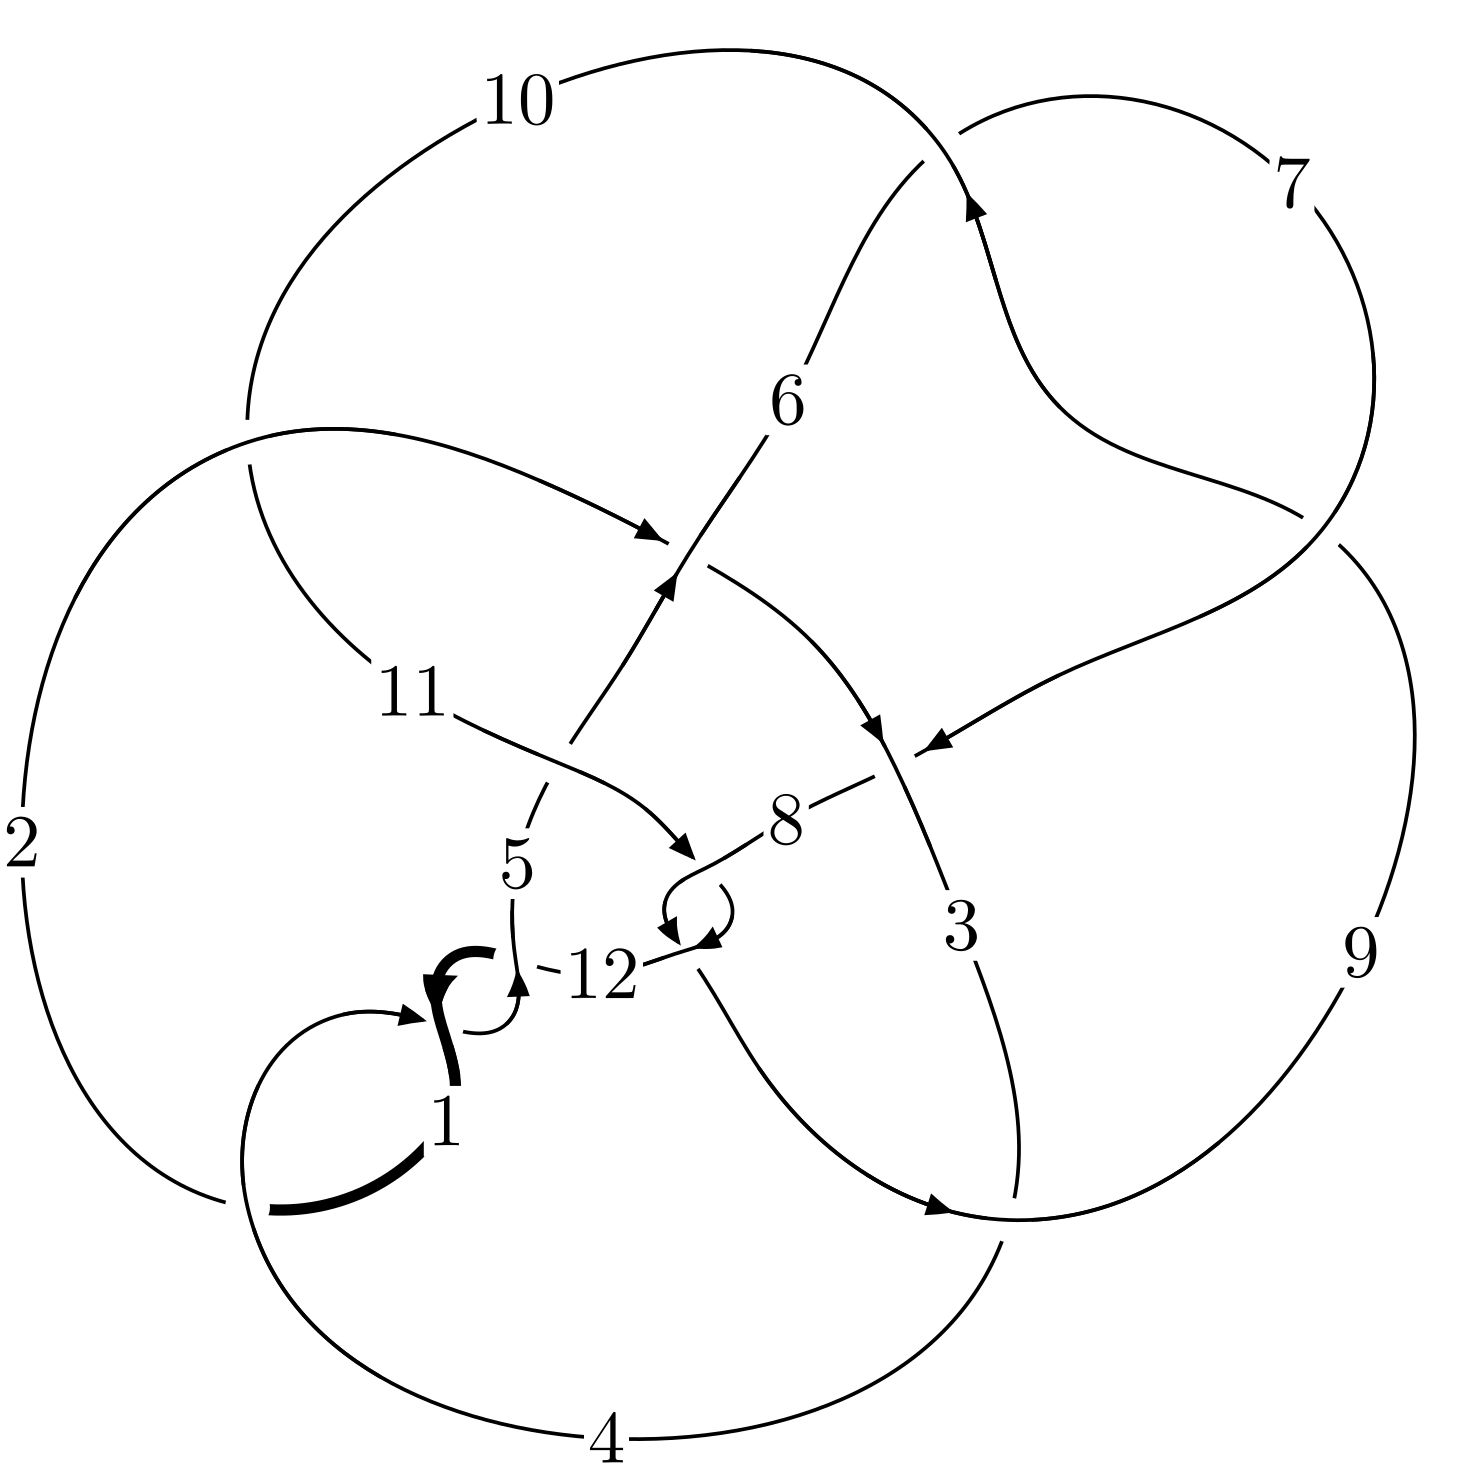
\includegraphics[width=112pt]{../../../GIT/diagram.site/Diagrams/png/1744_12a_0943.png}\\
\ \ \ A knot diagram\footnotemark}&
\allowdisplaybreaks
\textbf{Linearized knot diagam} \\
\cline{2-2}
 &
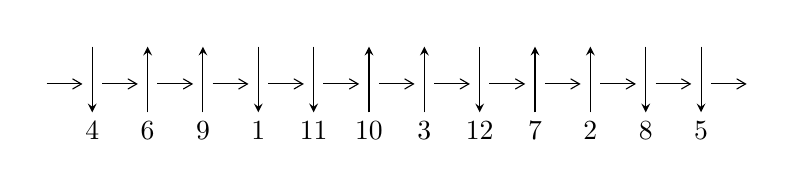
\begin{tikzpicture}[x=20pt, y=17pt]
	% nodes
	\node (C0) at (0, 0) {};
	\node (C1) at (1, 0) {};
	\node (C1U) at (1, +1) {};
	\node (C1D) at (1, -1) {4};

	\node (C2) at (2, 0) {};
	\node (C2U) at (2, +1) {};
	\node (C2D) at (2, -1) {6};

	\node (C3) at (3, 0) {};
	\node (C3U) at (3, +1) {};
	\node (C3D) at (3, -1) {9};

	\node (C4) at (4, 0) {};
	\node (C4U) at (4, +1) {};
	\node (C4D) at (4, -1) {1};

	\node (C5) at (5, 0) {};
	\node (C5U) at (5, +1) {};
	\node (C5D) at (5, -1) {11};

	\node (C6) at (6, 0) {};
	\node (C6U) at (6, +1) {};
	\node (C6D) at (6, -1) {10};

	\node (C7) at (7, 0) {};
	\node (C7U) at (7, +1) {};
	\node (C7D) at (7, -1) {3};

	\node (C8) at (8, 0) {};
	\node (C8U) at (8, +1) {};
	\node (C8D) at (8, -1) {12};

	\node (C9) at (9, 0) {};
	\node (C9U) at (9, +1) {};
	\node (C9D) at (9, -1) {7};

	\node (C10) at (10, 0) {};
	\node (C10U) at (10, +1) {};
	\node (C10D) at (10, -1) {2};

	\node (C11) at (11, 0) {};
	\node (C11U) at (11, +1) {};
	\node (C11D) at (11, -1) {8};

	\node (C12) at (12, 0) {};
	\node (C12U) at (12, +1) {};
	\node (C12D) at (12, -1) {5};
	\node (C13) at (13, 0) {};

	% arrows
	\draw[->,>={angle 60}]
	(C0) edge (C1) (C1) edge (C2) (C2) edge (C3) (C3) edge (C4) (C4) edge (C5) (C5) edge (C6) (C6) edge (C7) (C7) edge (C8) (C8) edge (C9) (C9) edge (C10) (C10) edge (C11) (C11) edge (C12) (C12) edge (C13) ;	\draw[->,>=stealth]
	(C1U) edge (C1D) (C2D) edge (C2U) (C3D) edge (C3U) (C4U) edge (C4D) (C5U) edge (C5D) (C6D) edge (C6U) (C7D) edge (C7U) (C8U) edge (C8D) (C9D) edge (C9U) (C10D) edge (C10U) (C11U) edge (C11D) (C12U) edge (C12D) ;
	\end{tikzpicture} \\
\hhline{~~} \\& 
\textbf{Solving Sequence} \\ \cline{2-2} 
 &
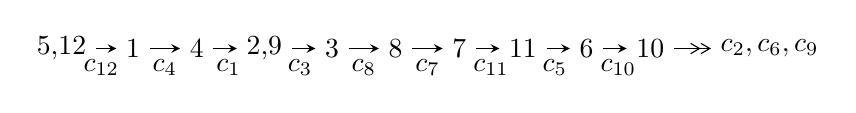
\begin{tikzpicture}[x=23pt, y=7pt]
	% node
	\node (A0) at (-1/8, 0) {5,12};
	\node (A1) at (1, 0) {1};
	\node (A2) at (2, 0) {4};
	\node (A3) at (49/16, 0) {2,9};
	\node (A4) at (33/8, 0) {3};
	\node (A5) at (41/8, 0) {8};
	\node (A6) at (49/8, 0) {7};
	\node (A7) at (57/8, 0) {11};
	\node (A8) at (65/8, 0) {6};
	\node (A9) at (73/8, 0) {10};
	\node (C1) at (1/2, -1) {$c_{12}$};
	\node (C2) at (3/2, -1) {$c_{4}$};
	\node (C3) at (5/2, -1) {$c_{1}$};
	\node (C4) at (29/8, -1) {$c_{3}$};
	\node (C5) at (37/8, -1) {$c_{8}$};
	\node (C6) at (45/8, -1) {$c_{7}$};
	\node (C7) at (53/8, -1) {$c_{11}$};
	\node (C8) at (61/8, -1) {$c_{5}$};
	\node (C9) at (69/8, -1) {$c_{10}$};
	\node (A10) at (11, 0) {$c_{2},c_{6},c_{9}$};

	% edge
	\draw[->,>=stealth]	
	(A0) edge (A1) (A1) edge (A2) (A2) edge (A3) (A3) edge (A4) (A4) edge (A5) (A5) edge (A6) (A6) edge (A7) (A7) edge (A8) (A8) edge (A9) ;
	\draw[->>,>={angle 60}]	
	(A9) edge (A10);
\end{tikzpicture} \\ 

\end{tabular} \\

\footnotetext{
The image of knot diagram is generated by the software ``\textbf{Draw programme}" developed by Andrew Bartholomew(\url{http://www.layer8.co.uk/maths/draw/index.htm\#Running-draw}), where we modified some parts for our purpose(\url{https://github.com/CATsTAILs/LinksPainter}).
}\phantom \\ \newline 
\centering \textbf{Ideals for irreducible components\footnotemark of $X_{\text{par}}$} 
 
\begin{align*}
I^u_{1}&=\langle 
1.78712\times10^{517} u^{145}-1.33819\times10^{518} u^{144}+\cdots+6.78869\times10^{518} b-5.80111\times10^{518},\\
\phantom{I^u_{1}}&\phantom{= \langle  }-1.40605\times10^{519} u^{145}+1.05376\times10^{520} u^{144}+\cdots+2.10450\times10^{520} a-9.14715\times10^{520},\\
\phantom{I^u_{1}}&\phantom{= \langle  }u^{146}-7 u^{145}+\cdots+117 u+31\rangle \\
I^u_{2}&=\langle 
150001 u^{35}+1354688 u^{34}+\cdots+891921 b+1011631,\\
\phantom{I^u_{2}}&\phantom{= \langle  }-918644 u^{35}+3557286 u^{34}+\cdots+891921 a-2376240,\;u^{36}-8 u^{35}+\cdots-10 u+1\rangle \\
\\
\end{align*}
\raggedright * 2 irreducible components of $\dim_{\mathbb{C}}=0$, with total 182 representations.\\
\footnotetext{All coefficients of polynomials are rational numbers. But the coefficients are sometimes approximated in decimal forms when there is not enough margin.}
\newpage
\renewcommand{\arraystretch}{1}
\centering \section*{I. $I^u_{1}= \langle 1.79\times10^{517} u^{145}-1.34\times10^{518} u^{144}+\cdots+6.79\times10^{518} b-5.80\times10^{518},\;-1.41\times10^{519} u^{145}+1.05\times10^{520} u^{144}+\cdots+2.10\times10^{520} a-9.15\times10^{520},\;u^{146}-7 u^{145}+\cdots+117 u+31 \rangle$}
\flushleft \textbf{(i) Arc colorings}\\
\begin{tabular}{m{7pt} m{180pt} m{7pt} m{180pt} }
\flushright $a_{5}=$&$\begin{pmatrix}0\\u\end{pmatrix}$ \\
\flushright $a_{12}=$&$\begin{pmatrix}1\\0\end{pmatrix}$ \\
\flushright $a_{1}=$&$\begin{pmatrix}1\\u^2\end{pmatrix}$ \\
\flushright $a_{4}=$&$\begin{pmatrix}u\\u^3+u\end{pmatrix}$ \\
\flushright $a_{2}=$&$\begin{pmatrix}u^2+1\\u^4+2 u^2\end{pmatrix}$ \\
\flushright $a_{9}=$&$\begin{pmatrix}0.0668117 u^{145}-0.500717 u^{144}+\cdots-26.7482 u+4.34648\\-0.0263250 u^{145}+0.197120 u^{144}+\cdots-1.04940 u+0.854525\end{pmatrix}$ \\
\flushright $a_{3}=$&$\begin{pmatrix}-0.0108550 u^{145}+0.121391 u^{144}+\cdots-16.3069 u+3.52191\\0.0207079 u^{145}-0.149856 u^{144}+\cdots-2.81401 u-0.238209\end{pmatrix}$ \\
\flushright $a_{8}=$&$\begin{pmatrix}0.0404867 u^{145}-0.303596 u^{144}+\cdots-27.7976 u+5.20101\\-0.0263250 u^{145}+0.197120 u^{144}+\cdots-1.04940 u+0.854525\end{pmatrix}$ \\
\flushright $a_{7}=$&$\begin{pmatrix}0.0558723 u^{145}-0.372603 u^{144}+\cdots-3.26923 u+2.17630\\-0.0251010 u^{145}+0.179971 u^{144}+\cdots+1.78696 u+0.577547\end{pmatrix}$ \\
\flushright $a_{11}=$&$\begin{pmatrix}0.00181010 u^{145}-0.0179139 u^{144}+\cdots+20.7607 u-1.65983\\-0.00208124 u^{145}-0.0464347 u^{144}+\cdots+1.81185 u-0.736714\end{pmatrix}$ \\
\flushright $a_{6}=$&$\begin{pmatrix}-0.0159414 u^{145}+0.110964 u^{144}+\cdots+7.43670 u-4.92878\\-0.0176368 u^{145}+0.114351 u^{144}+\cdots+4.21484 u-0.761534\end{pmatrix}$ \\
\flushright $a_{10}=$&$\begin{pmatrix}0.00715498 u^{145}-0.0371041 u^{144}+\cdots+15.7315 u-1.64989\\-0.00307858 u^{145}-0.0206540 u^{144}+\cdots+3.24478 u-0.384611\end{pmatrix}$\\&\end{tabular}
\flushleft \textbf{(ii) Obstruction class $= -1$}\\~\\
\flushleft \textbf{(iii) Cusp Shapes $= -0.240462 u^{145}+1.85632 u^{144}+\cdots+5.56279 u-3.36132$}\\~\\
\newpage\renewcommand{\arraystretch}{1}
\flushleft \textbf{(iv) u-Polynomials at the component}\newline \\
\begin{tabular}{m{50pt}|m{274pt}}
Crossings & \hspace{64pt}u-Polynomials at each crossing \\
\hline $$\begin{aligned}c_{1},c_{4},c_{12}\end{aligned}$$&$\begin{aligned}
&u^{146}+7 u^{145}+\cdots-117 u+31
\end{aligned}$\\
\hline $$\begin{aligned}c_{2}\end{aligned}$$&$\begin{aligned}
&u^{146}-3 u^{145}+\cdots-232 u+23
\end{aligned}$\\
\hline $$\begin{aligned}c_{3}\end{aligned}$$&$\begin{aligned}
&u^{146}- u^{145}+\cdots+36926312 u+87096208
\end{aligned}$\\
\hline $$\begin{aligned}c_{5}\end{aligned}$$&$\begin{aligned}
&u^{146}+u^{145}+\cdots-73218680 u+5055088
\end{aligned}$\\
\hline $$\begin{aligned}c_{6},c_{9}\end{aligned}$$&$\begin{aligned}
&u^{146}+6 u^{145}+\cdots+59 u+1
\end{aligned}$\\
\hline $$\begin{aligned}c_{7}\end{aligned}$$&$\begin{aligned}
&u^{146}+14 u^{144}+\cdots-34304 u+1984
\end{aligned}$\\
\hline $$\begin{aligned}c_{8},c_{11}\end{aligned}$$&$\begin{aligned}
&u^{146}+6 u^{145}+\cdots+10735 u+2329
\end{aligned}$\\
\hline $$\begin{aligned}c_{10}\end{aligned}$$&$\begin{aligned}
&u^{146}-6 u^{145}+\cdots+186624 u+155392
\end{aligned}$\\
\hline
\end{tabular}\\~\\
\newpage\renewcommand{\arraystretch}{1}
\flushleft \textbf{(v) Riley Polynomials at the component}\newline \\
\begin{tabular}{m{50pt}|m{274pt}}
Crossings & \hspace{64pt}Riley Polynomials at each crossing \\
\hline $$\begin{aligned}c_{1},c_{4},c_{12}\end{aligned}$$&$\begin{aligned}
&y^{146}+139 y^{145}+\cdots-122499 y+961
\end{aligned}$\\
\hline $$\begin{aligned}c_{2}\end{aligned}$$&$\begin{aligned}
&y^{146}+21 y^{145}+\cdots+34036 y+529
\end{aligned}$\\
\hline $$\begin{aligned}c_{3}\end{aligned}$$&$\begin{aligned}
&y^{146}+25 y^{145}+\cdots+222241981535540160 y+7585749447979264
\end{aligned}$\\
\hline $$\begin{aligned}c_{5}\end{aligned}$$&$\begin{aligned}
&y^{146}+29 y^{145}+\cdots+948957128361152 y+25553914687744
\end{aligned}$\\
\hline $$\begin{aligned}c_{6},c_{9}\end{aligned}$$&$\begin{aligned}
&y^{146}+104 y^{145}+\cdots-243 y+1
\end{aligned}$\\
\hline $$\begin{aligned}c_{7}\end{aligned}$$&$\begin{aligned}
&y^{146}+28 y^{145}+\cdots+135151616 y+3936256
\end{aligned}$\\
\hline $$\begin{aligned}c_{8},c_{11}\end{aligned}$$&$\begin{aligned}
&y^{146}-76 y^{145}+\cdots-142242651 y+5424241
\end{aligned}$\\
\hline $$\begin{aligned}c_{10}\end{aligned}$$&$\begin{aligned}
&y^{146}+20 y^{145}+\cdots+1419362140160 y+24146673664
\end{aligned}$\\
\hline
\end{tabular}\\~\\
\newpage\flushleft \textbf{(vi) Complex Volumes and Cusp Shapes}
$$\begin{array}{c|c|c}  
\text{Solutions to }I^u_{1}& \I (\text{vol} + \sqrt{-1}CS) & \text{Cusp shape}\\
 \hline 
\begin{aligned}
u &= -0.600308 + 0.786562 I \\
a &= \phantom{-}0.263013 - 0.319264 I \\
b &= -1.055520 - 0.453993 I\end{aligned}
 & \phantom{-}0.29286 - 4.41022 I & \phantom{-0.000000 } 0 \\ \hline\begin{aligned}
u &= -0.600308 - 0.786562 I \\
a &= \phantom{-}0.263013 + 0.319264 I \\
b &= -1.055520 + 0.453993 I\end{aligned}
 & \phantom{-}0.29286 + 4.41022 I & \phantom{-0.000000 } 0 \\ \hline\begin{aligned}
u &= \phantom{-}0.710381 + 0.675563 I \\
a &= -0.160649 + 0.663844 I \\
b &= -1.239970 - 0.424123 I\end{aligned}
 & -4.13553 - 5.87181 I & \phantom{-0.000000 } 0 \\ \hline\begin{aligned}
u &= \phantom{-}0.710381 - 0.675563 I \\
a &= -0.160649 - 0.663844 I \\
b &= -1.239970 + 0.424123 I\end{aligned}
 & -4.13553 + 5.87181 I & \phantom{-0.000000 } 0 \\ \hline\begin{aligned}
u &= -0.950755 + 0.378156 I \\
a &= \phantom{-}0.576510 + 0.789498 I \\
b &= \phantom{-}1.220860 - 0.595168 I\end{aligned}
 & -5.8255 + 14.7586 I & \phantom{-0.000000 } 0 \\ \hline\begin{aligned}
u &= -0.950755 - 0.378156 I \\
a &= \phantom{-}0.576510 - 0.789498 I \\
b &= \phantom{-}1.220860 + 0.595168 I\end{aligned}
 & -5.8255 - 14.7586 I & \phantom{-0.000000 } 0 \\ \hline\begin{aligned}
u &= \phantom{-}0.876850 + 0.401996 I \\
a &= -0.657246 + 0.667423 I \\
b &= -1.059220 - 0.374861 I\end{aligned}
 & -2.73674 - 3.81103 I & \phantom{-0.000000 } 0 \\ \hline\begin{aligned}
u &= \phantom{-}0.876850 - 0.401996 I \\
a &= -0.657246 - 0.667423 I \\
b &= -1.059220 + 0.374861 I\end{aligned}
 & -2.73674 + 3.81103 I & \phantom{-0.000000 } 0 \\ \hline\begin{aligned}
u &= \phantom{-}0.920571 + 0.263564 I \\
a &= -0.342320 + 0.713848 I \\
b &= -1.005740 + 0.168942 I\end{aligned}
 & -5.52437 + 0.55845 I & \phantom{-0.000000 } 0 \\ \hline\begin{aligned}
u &= \phantom{-}0.920571 - 0.263564 I \\
a &= -0.342320 - 0.713848 I \\
b &= -1.005740 - 0.168942 I\end{aligned}
 & -5.52437 - 0.55845 I & \phantom{-0.000000 } 0\\
 \hline 
 \end{array}$$\newpage$$\begin{array}{c|c|c}  
\text{Solutions to }I^u_{1}& \I (\text{vol} + \sqrt{-1}CS) & \text{Cusp shape}\\
 \hline 
\begin{aligned}
u &= \phantom{-}0.248446 + 1.032260 I \\
a &= \phantom{-}0.05791 + 2.36671 I \\
b &= -0.773771 - 0.599814 I\end{aligned}
 & -2.70153 - 6.27133 I & \phantom{-0.000000 } 0 \\ \hline\begin{aligned}
u &= \phantom{-}0.248446 - 1.032260 I \\
a &= \phantom{-}0.05791 - 2.36671 I \\
b &= -0.773771 + 0.599814 I\end{aligned}
 & -2.70153 + 6.27133 I & \phantom{-0.000000 } 0 \\ \hline\begin{aligned}
u &= \phantom{-}0.927301 + 0.037439 I \\
a &= -0.456936 - 0.740794 I \\
b &= -0.972638 + 0.460098 I\end{aligned}
 & -5.63011 + 1.69117 I & \phantom{-0.000000 } 0 \\ \hline\begin{aligned}
u &= \phantom{-}0.927301 - 0.037439 I \\
a &= -0.456936 + 0.740794 I \\
b &= -0.972638 - 0.460098 I\end{aligned}
 & -5.63011 - 1.69117 I & \phantom{-0.000000 } 0 \\ \hline\begin{aligned}
u &= -0.823585 + 0.343442 I \\
a &= -0.766504 - 0.808831 I \\
b &= -1.228460 + 0.594830 I\end{aligned}
 & -1.10225 + 9.30326 I & \phantom{-0.000000 } 0 \\ \hline\begin{aligned}
u &= -0.823585 - 0.343442 I \\
a &= -0.766504 + 0.808831 I \\
b &= -1.228460 - 0.594830 I\end{aligned}
 & -1.10225 - 9.30326 I & \phantom{-0.000000 } 0 \\ \hline\begin{aligned}
u &= \phantom{-}0.471973 + 0.755429 I \\
a &= \phantom{-}0.547287 - 0.692286 I \\
b &= -0.452214 + 0.309658 I\end{aligned}
 & -2.03687 - 2.78273 I & \phantom{-0.000000 } 0 \\ \hline\begin{aligned}
u &= \phantom{-}0.471973 - 0.755429 I \\
a &= \phantom{-}0.547287 + 0.692286 I \\
b &= -0.452214 - 0.309658 I\end{aligned}
 & -2.03687 + 2.78273 I & \phantom{-0.000000 } 0 \\ \hline\begin{aligned}
u &= \phantom{-}1.058890 + 0.388787 I \\
a &= \phantom{-}0.412535 - 0.239057 I \\
b &= \phantom{-}1.133490 + 0.285129 I\end{aligned}
 & -5.98452 - 3.86162 I & \phantom{-0.000000 } 0 \\ \hline\begin{aligned}
u &= \phantom{-}1.058890 - 0.388787 I \\
a &= \phantom{-}0.412535 + 0.239057 I \\
b &= \phantom{-}1.133490 - 0.285129 I\end{aligned}
 & -5.98452 + 3.86162 I & \phantom{-0.000000 } 0\\
 \hline 
 \end{array}$$\newpage$$\begin{array}{c|c|c}  
\text{Solutions to }I^u_{1}& \I (\text{vol} + \sqrt{-1}CS) & \text{Cusp shape}\\
 \hline 
\begin{aligned}
u &= \phantom{-}1.035090 + 0.463986 I \\
a &= \phantom{-}0.471933 - 0.959842 I \\
b &= \phantom{-}1.027660 + 0.425622 I\end{aligned}
 & -5.72968 - 4.48341 I & \phantom{-0.000000 } 0 \\ \hline\begin{aligned}
u &= \phantom{-}1.035090 - 0.463986 I \\
a &= \phantom{-}0.471933 + 0.959842 I \\
b &= \phantom{-}1.027660 - 0.425622 I\end{aligned}
 & -5.72968 + 4.48341 I & \phantom{-0.000000 } 0 \\ \hline\begin{aligned}
u &= -0.076786 + 1.154700 I \\
a &= \phantom{-}0.144743 + 0.110076 I \\
b &= -1.48191 - 0.22697 I\end{aligned}
 & -5.32053 - 4.44523 I & \phantom{-0.000000 } 0 \\ \hline\begin{aligned}
u &= -0.076786 - 1.154700 I \\
a &= \phantom{-}0.144743 - 0.110076 I \\
b &= -1.48191 + 0.22697 I\end{aligned}
 & -5.32053 + 4.44523 I & \phantom{-0.000000 } 0 \\ \hline\begin{aligned}
u &= \phantom{-}0.673070 + 0.943463 I \\
a &= -0.097615 + 0.277155 I \\
b &= -0.855254 + 0.159813 I\end{aligned}
 & -1.22395 - 1.64245 I & \phantom{-0.000000 } 0 \\ \hline\begin{aligned}
u &= \phantom{-}0.673070 - 0.943463 I \\
a &= -0.097615 - 0.277155 I \\
b &= -0.855254 - 0.159813 I\end{aligned}
 & -1.22395 + 1.64245 I & \phantom{-0.000000 } 0 \\ \hline\begin{aligned}
u &= -0.604200 + 0.546499 I \\
a &= \phantom{-}1.45515 + 0.62412 I \\
b &= \phantom{-}0.413674 - 0.463374 I\end{aligned}
 & -2.21578 - 4.91795 I & \phantom{-0.000000 } 0 \\ \hline\begin{aligned}
u &= -0.604200 - 0.546499 I \\
a &= \phantom{-}1.45515 - 0.62412 I \\
b &= \phantom{-}0.413674 + 0.463374 I\end{aligned}
 & -2.21578 + 4.91795 I & \phantom{-0.000000 } 0 \\ \hline\begin{aligned}
u &= -0.697511 + 0.374057 I \\
a &= \phantom{-}0.153012 - 0.426392 I \\
b &= \phantom{-}0.234013 + 0.975605 I\end{aligned}
 & -2.81738 + 9.12644 I & \phantom{-0.000000 } 0 \\ \hline\begin{aligned}
u &= -0.697511 - 0.374057 I \\
a &= \phantom{-}0.153012 + 0.426392 I \\
b &= \phantom{-}0.234013 - 0.975605 I\end{aligned}
 & -2.81738 - 9.12644 I & \phantom{-0.000000 } 0\\
 \hline 
 \end{array}$$\newpage$$\begin{array}{c|c|c}  
\text{Solutions to }I^u_{1}& \I (\text{vol} + \sqrt{-1}CS) & \text{Cusp shape}\\
 \hline 
\begin{aligned}
u &= -0.780473 + 0.927697 I \\
a &= -0.280900 + 0.109842 I \\
b &= \phantom{-}1.081760 + 0.471945 I\end{aligned}
 & -4.24779 - 8.88674 I & \phantom{-0.000000 } 0 \\ \hline\begin{aligned}
u &= -0.780473 - 0.927697 I \\
a &= -0.280900 - 0.109842 I \\
b &= \phantom{-}1.081760 - 0.471945 I\end{aligned}
 & -4.24779 + 8.88674 I & \phantom{-0.000000 } 0 \\ \hline\begin{aligned}
u &= \phantom{-}0.821779 + 0.895107 I \\
a &= \phantom{-}0.253931 + 0.215585 I \\
b &= \phantom{-}0.878324 - 0.273970 I\end{aligned}
 & -4.54611 - 1.90325 I & \phantom{-0.000000 } 0 \\ \hline\begin{aligned}
u &= \phantom{-}0.821779 - 0.895107 I \\
a &= \phantom{-}0.253931 - 0.215585 I \\
b &= \phantom{-}0.878324 + 0.273970 I\end{aligned}
 & -4.54611 + 1.90325 I & \phantom{-0.000000 } 0 \\ \hline\begin{aligned}
u &= \phantom{-}0.448782 + 1.129800 I \\
a &= \phantom{-}0.282045 - 0.326218 I \\
b &= -0.968796 + 0.200248 I\end{aligned}
 & -2.09122 - 3.25336 I & \phantom{-0.000000 } 0 \\ \hline\begin{aligned}
u &= \phantom{-}0.448782 - 1.129800 I \\
a &= \phantom{-}0.282045 + 0.326218 I \\
b &= -0.968796 - 0.200248 I\end{aligned}
 & -2.09122 + 3.25336 I & \phantom{-0.000000 } 0 \\ \hline\begin{aligned}
u &= -0.287540 + 1.188040 I \\
a &= -0.894690 + 0.350012 I \\
b &= \phantom{-}1.329140 + 0.452737 I\end{aligned}
 & -1.37349 + 0.92683 I & \phantom{-0.000000 } 0 \\ \hline\begin{aligned}
u &= -0.287540 - 1.188040 I \\
a &= -0.894690 - 0.350012 I \\
b &= \phantom{-}1.329140 - 0.452737 I\end{aligned}
 & -1.37349 - 0.92683 I & \phantom{-0.000000 } 0 \\ \hline\begin{aligned}
u &= -0.030401 + 1.243270 I \\
a &= \phantom{-}0.21021 + 2.56463 I \\
b &= -0.641198 - 0.258051 I\end{aligned}
 & -0.68606 + 6.01802 I & \phantom{-0.000000 } 0 \\ \hline\begin{aligned}
u &= -0.030401 - 1.243270 I \\
a &= \phantom{-}0.21021 - 2.56463 I \\
b &= -0.641198 + 0.258051 I\end{aligned}
 & -0.68606 - 6.01802 I & \phantom{-0.000000 } 0\\
 \hline 
 \end{array}$$\newpage$$\begin{array}{c|c|c}  
\text{Solutions to }I^u_{1}& \I (\text{vol} + \sqrt{-1}CS) & \text{Cusp shape}\\
 \hline 
\begin{aligned}
u &= -0.098424 + 1.241790 I \\
a &= -0.621581 + 0.389280 I \\
b &= \phantom{-}1.54433 + 0.04239 I\end{aligned}
 & -0.45702 + 1.43647 I & \phantom{-0.000000 } 0 \\ \hline\begin{aligned}
u &= -0.098424 - 1.241790 I \\
a &= -0.621581 - 0.389280 I \\
b &= \phantom{-}1.54433 - 0.04239 I\end{aligned}
 & -0.45702 - 1.43647 I & \phantom{-0.000000 } 0 \\ \hline\begin{aligned}
u &= -0.733155 + 0.092657 I \\
a &= \phantom{-}1.016870 + 0.296987 I \\
b &= \phantom{-}1.26236 - 0.68131 I\end{aligned}
 & -4.69874 + 2.79612 I & \phantom{-0.000000 } 0 \\ \hline\begin{aligned}
u &= -0.733155 - 0.092657 I \\
a &= \phantom{-}1.016870 - 0.296987 I \\
b &= \phantom{-}1.26236 + 0.68131 I\end{aligned}
 & -4.69874 - 2.79612 I & \phantom{-0.000000 } 0 \\ \hline\begin{aligned}
u &= \phantom{-}0.663880 + 0.311056 I \\
a &= -0.018267 + 0.881601 I \\
b &= \phantom{-}0.090419 - 0.426726 I\end{aligned}
 & -3.45989 - 1.16177 I & \phantom{-0.000000 } 0 \\ \hline\begin{aligned}
u &= \phantom{-}0.663880 - 0.311056 I \\
a &= -0.018267 - 0.881601 I \\
b &= \phantom{-}0.090419 + 0.426726 I\end{aligned}
 & -3.45989 + 1.16177 I & \phantom{-0.000000 } 0 \\ \hline\begin{aligned}
u &= \phantom{-}0.363362 + 0.635871 I \\
a &= -1.221540 - 0.420107 I \\
b &= \phantom{-}0.925861 - 0.197907 I\end{aligned}
 & -0.153349 - 0.132354 I & \phantom{-0.000000 } 0 \\ \hline\begin{aligned}
u &= \phantom{-}0.363362 - 0.635871 I \\
a &= -1.221540 + 0.420107 I \\
b &= \phantom{-}0.925861 + 0.197907 I\end{aligned}
 & -0.153349 + 0.132354 I & \phantom{-0.000000 } 0 \\ \hline\begin{aligned}
u &= -0.056699 + 1.274890 I \\
a &= -0.89526 - 2.10953 I \\
b &= \phantom{-}0.362918 + 1.164050 I\end{aligned}
 & \phantom{-}4.42784 - 2.41245 I & \phantom{-0.000000 } 0 \\ \hline\begin{aligned}
u &= -0.056699 - 1.274890 I \\
a &= -0.89526 + 2.10953 I \\
b &= \phantom{-}0.362918 - 1.164050 I\end{aligned}
 & \phantom{-}4.42784 + 2.41245 I & \phantom{-0.000000 } 0\\
 \hline 
 \end{array}$$\newpage$$\begin{array}{c|c|c}  
\text{Solutions to }I^u_{1}& \I (\text{vol} + \sqrt{-1}CS) & \text{Cusp shape}\\
 \hline 
\begin{aligned}
u &= \phantom{-}0.112257 + 1.278830 I \\
a &= -0.19799 - 2.06823 I \\
b &= \phantom{-}0.662336 + 0.119214 I\end{aligned}
 & \phantom{-}3.48220 + 0.33660 I & \phantom{-0.000000 } 0 \\ \hline\begin{aligned}
u &= \phantom{-}0.112257 - 1.278830 I \\
a &= -0.19799 + 2.06823 I \\
b &= \phantom{-}0.662336 - 0.119214 I\end{aligned}
 & \phantom{-}3.48220 - 0.33660 I & \phantom{-0.000000 } 0 \\ \hline\begin{aligned}
u &= \phantom{-}0.358917 + 0.615524 I \\
a &= -1.26873 + 2.55917 I \\
b &= -0.834546 - 0.388384 I\end{aligned}
 & -2.83699 - 6.20686 I & \phantom{-0.000000 -}0. + 10.87479 I \\ \hline\begin{aligned}
u &= \phantom{-}0.358917 - 0.615524 I \\
a &= -1.26873 - 2.55917 I \\
b &= -0.834546 + 0.388384 I\end{aligned}
 & -2.83699 + 6.20686 I & \phantom{-0.000000 } 0. - 10.87479 I \\ \hline\begin{aligned}
u &= -0.139703 + 1.284050 I \\
a &= \phantom{-}0.872531 - 0.086241 I \\
b &= -1.71657 - 0.09524 I\end{aligned}
 & -4.66332 + 7.15556 I & \phantom{-0.000000 } 0 \\ \hline\begin{aligned}
u &= -0.139703 - 1.284050 I \\
a &= \phantom{-}0.872531 + 0.086241 I \\
b &= -1.71657 + 0.09524 I\end{aligned}
 & -4.66332 - 7.15556 I & \phantom{-0.000000 } 0 \\ \hline\begin{aligned}
u &= -0.223759 + 1.274350 I \\
a &= \phantom{-}0.92487 - 1.66131 I \\
b &= -1.097840 + 0.493168 I\end{aligned}
 & -4.16337 - 1.87122 I & \phantom{-0.000000 } 0 \\ \hline\begin{aligned}
u &= -0.223759 - 1.274350 I \\
a &= \phantom{-}0.92487 + 1.66131 I \\
b &= -1.097840 - 0.493168 I\end{aligned}
 & -4.16337 + 1.87122 I & \phantom{-0.000000 } 0 \\ \hline\begin{aligned}
u &= \phantom{-}0.040291 + 1.295820 I \\
a &= \phantom{-}0.23230 - 1.76775 I \\
b &= -1.133660 + 0.662083 I\end{aligned}
 & \phantom{-}1.87406 + 1.51346 I & \phantom{-0.000000 } 0 \\ \hline\begin{aligned}
u &= \phantom{-}0.040291 - 1.295820 I \\
a &= \phantom{-}0.23230 + 1.76775 I \\
b &= -1.133660 - 0.662083 I\end{aligned}
 & \phantom{-}1.87406 - 1.51346 I & \phantom{-0.000000 } 0\\
 \hline 
 \end{array}$$\newpage$$\begin{array}{c|c|c}  
\text{Solutions to }I^u_{1}& \I (\text{vol} + \sqrt{-1}CS) & \text{Cusp shape}\\
 \hline 
\begin{aligned}
u &= -0.322674 + 1.257330 I \\
a &= \phantom{-}0.76820 + 1.63579 I \\
b &= \phantom{-}0.668901 - 0.810258 I\end{aligned}
 & \phantom{-}1.14020 + 7.00435 I & \phantom{-0.000000 } 0 \\ \hline\begin{aligned}
u &= -0.322674 - 1.257330 I \\
a &= \phantom{-}0.76820 - 1.63579 I \\
b &= \phantom{-}0.668901 + 0.810258 I\end{aligned}
 & \phantom{-}1.14020 - 7.00435 I & \phantom{-0.000000 } 0 \\ \hline\begin{aligned}
u &= \phantom{-}0.909914 + 0.968779 I \\
a &= -0.015212 - 0.506982 I \\
b &= \phantom{-}0.908547 - 0.078071 I\end{aligned}
 & -4.41947 - 2.76812 I & \phantom{-0.000000 } 0 \\ \hline\begin{aligned}
u &= \phantom{-}0.909914 - 0.968779 I \\
a &= -0.015212 + 0.506982 I \\
b &= \phantom{-}0.908547 + 0.078071 I\end{aligned}
 & -4.41947 + 2.76812 I & \phantom{-0.000000 } 0 \\ \hline\begin{aligned}
u &= -0.191254 + 1.326680 I \\
a &= -0.788587 - 0.960048 I \\
b &= \phantom{-}0.566130 + 1.028180 I\end{aligned}
 & \phantom{-}1.62293 - 0.45548 I & \phantom{-0.000000 } 0 \\ \hline\begin{aligned}
u &= -0.191254 - 1.326680 I \\
a &= -0.788587 + 0.960048 I \\
b &= \phantom{-}0.566130 - 1.028180 I\end{aligned}
 & \phantom{-}1.62293 + 0.45548 I & \phantom{-0.000000 } 0 \\ \hline\begin{aligned}
u &= -0.658028 + 0.033714 I \\
a &= \phantom{-}0.860356 - 0.040788 I \\
b &= \phantom{-}0.487871 + 0.818994 I\end{aligned}
 & -2.60226 - 3.36266 I & -2.88422 + 8.32461 I \\ \hline\begin{aligned}
u &= -0.658028 - 0.033714 I \\
a &= \phantom{-}0.860356 + 0.040788 I \\
b &= \phantom{-}0.487871 - 0.818994 I\end{aligned}
 & -2.60226 + 3.36266 I & -2.88422 - 8.32461 I \\ \hline\begin{aligned}
u &= \phantom{-}0.590138 + 0.292913 I \\
a &= \phantom{-}0.349197 - 0.886307 I \\
b &= \phantom{-}1.124890 + 0.561726 I\end{aligned}
 & -1.38197 - 3.16972 I & \phantom{-}0.24009 + 5.86421 I \\ \hline\begin{aligned}
u &= \phantom{-}0.590138 - 0.292913 I \\
a &= \phantom{-}0.349197 + 0.886307 I \\
b &= \phantom{-}1.124890 - 0.561726 I\end{aligned}
 & -1.38197 + 3.16972 I & \phantom{-}0.24009 - 5.86421 I\\
 \hline 
 \end{array}$$\newpage$$\begin{array}{c|c|c}  
\text{Solutions to }I^u_{1}& \I (\text{vol} + \sqrt{-1}CS) & \text{Cusp shape}\\
 \hline 
\begin{aligned}
u &= -0.544271 + 0.322218 I \\
a &= \phantom{-}0.002303 + 0.176521 I \\
b &= -0.231322 - 1.018080 I\end{aligned}
 & \phantom{-}1.97463 + 3.59000 I & \phantom{-}2.18111 - 9.54008 I \\ \hline\begin{aligned}
u &= -0.544271 - 0.322218 I \\
a &= \phantom{-}0.002303 - 0.176521 I \\
b &= -0.231322 + 1.018080 I\end{aligned}
 & \phantom{-}1.97463 - 3.59000 I & \phantom{-}2.18111 + 9.54008 I \\ \hline\begin{aligned}
u &= -0.300405 + 1.336520 I \\
a &= -0.00901 + 1.91153 I \\
b &= \phantom{-}1.25841 - 0.84764 I\end{aligned}
 & -0.19380 + 6.52936 I & \phantom{-0.000000 } 0 \\ \hline\begin{aligned}
u &= -0.300405 - 1.336520 I \\
a &= -0.00901 - 1.91153 I \\
b &= \phantom{-}1.25841 + 0.84764 I\end{aligned}
 & -0.19380 - 6.52936 I & \phantom{-0.000000 } 0 \\ \hline\begin{aligned}
u &= -0.161418 + 1.363690 I \\
a &= -0.79148 + 1.80977 I \\
b &= \phantom{-}1.152160 - 0.449182 I\end{aligned}
 & \phantom{-}0.93742 + 2.88356 I & \phantom{-0.000000 } 0 \\ \hline\begin{aligned}
u &= -0.161418 - 1.363690 I \\
a &= -0.79148 - 1.80977 I \\
b &= \phantom{-}1.152160 + 0.449182 I\end{aligned}
 & \phantom{-}0.93742 - 2.88356 I & \phantom{-0.000000 } 0 \\ \hline\begin{aligned}
u &= -0.031138 + 1.374080 I \\
a &= -0.33165 + 1.64163 I \\
b &= \phantom{-}1.164800 - 0.613479 I\end{aligned}
 & \phantom{-}2.98509 + 2.56355 I & \phantom{-0.000000 } 0 \\ \hline\begin{aligned}
u &= -0.031138 - 1.374080 I \\
a &= -0.33165 - 1.64163 I \\
b &= \phantom{-}1.164800 + 0.613479 I\end{aligned}
 & \phantom{-}2.98509 - 2.56355 I & \phantom{-0.000000 } 0 \\ \hline\begin{aligned}
u &= \phantom{-}0.075398 + 1.381720 I \\
a &= -0.64377 + 1.75561 I \\
b &= \phantom{-}0.76129 - 1.35490 I\end{aligned}
 & \phantom{-}5.67006 + 1.62713 I & \phantom{-0.000000 } 0 \\ \hline\begin{aligned}
u &= \phantom{-}0.075398 - 1.381720 I \\
a &= -0.64377 - 1.75561 I \\
b &= \phantom{-}0.76129 + 1.35490 I\end{aligned}
 & \phantom{-}5.67006 - 1.62713 I & \phantom{-0.000000 } 0\\
 \hline 
 \end{array}$$\newpage$$\begin{array}{c|c|c}  
\text{Solutions to }I^u_{1}& \I (\text{vol} + \sqrt{-1}CS) & \text{Cusp shape}\\
 \hline 
\begin{aligned}
u &= \phantom{-}0.161331 + 1.386940 I \\
a &= \phantom{-}0.56011 - 1.32894 I \\
b &= \phantom{-}1.156120 + 0.345033 I\end{aligned}
 & \phantom{-}4.75595 - 4.27023 I & \phantom{-0.000000 } 0 \\ \hline\begin{aligned}
u &= \phantom{-}0.161331 - 1.386940 I \\
a &= \phantom{-}0.56011 + 1.32894 I \\
b &= \phantom{-}1.156120 - 0.345033 I\end{aligned}
 & \phantom{-}4.75595 + 4.27023 I & \phantom{-0.000000 } 0 \\ \hline\begin{aligned}
u &= \phantom{-}0.400753 + 1.355730 I \\
a &= \phantom{-}0.087799 + 0.999503 I \\
b &= -0.725981 - 0.034937 I\end{aligned}
 & -0.53523 - 4.19761 I & \phantom{-0.000000 } 0 \\ \hline\begin{aligned}
u &= \phantom{-}0.400753 - 1.355730 I \\
a &= \phantom{-}0.087799 - 0.999503 I \\
b &= -0.725981 + 0.034937 I\end{aligned}
 & -0.53523 + 4.19761 I & \phantom{-0.000000 } 0 \\ \hline\begin{aligned}
u &= -0.500335 + 0.300299 I \\
a &= -1.55821 - 0.36015 I \\
b &= -0.458401 + 0.490676 I\end{aligned}
 & \phantom{-}2.04668 - 0.50496 I & \phantom{-}4.74774 - 1.63481 I \\ \hline\begin{aligned}
u &= -0.500335 - 0.300299 I \\
a &= -1.55821 + 0.36015 I \\
b &= -0.458401 - 0.490676 I\end{aligned}
 & \phantom{-}2.04668 + 0.50496 I & \phantom{-}4.74774 + 1.63481 I \\ \hline\begin{aligned}
u &= -0.22933 + 1.41090 I \\
a &= -0.240214 - 1.348330 I \\
b &= -0.928330 + 0.600220 I\end{aligned}
 & \phantom{-}7.43972 + 2.33030 I & \phantom{-0.000000 } 0 \\ \hline\begin{aligned}
u &= -0.22933 - 1.41090 I \\
a &= -0.240214 + 1.348330 I \\
b &= -0.928330 - 0.600220 I\end{aligned}
 & \phantom{-}7.43972 - 2.33030 I & \phantom{-0.000000 } 0 \\ \hline\begin{aligned}
u &= -0.559237 + 0.068955 I \\
a &= -0.576035 - 1.250270 I \\
b &= -1.386620 + 0.233170 I\end{aligned}
 & -8.36721 - 4.78858 I & -9.12474 + 3.88127 I \\ \hline\begin{aligned}
u &= -0.559237 - 0.068955 I \\
a &= -0.576035 + 1.250270 I \\
b &= -1.386620 - 0.233170 I\end{aligned}
 & -8.36721 + 4.78858 I & -9.12474 - 3.88127 I\\
 \hline 
 \end{array}$$\newpage$$\begin{array}{c|c|c}  
\text{Solutions to }I^u_{1}& \I (\text{vol} + \sqrt{-1}CS) & \text{Cusp shape}\\
 \hline 
\begin{aligned}
u &= -0.21709 + 1.42007 I \\
a &= \phantom{-}0.74892 + 1.42849 I \\
b &= -0.418875 - 1.269480 I\end{aligned}
 & \phantom{-}7.54837 + 6.43308 I & \phantom{-0.000000 } 0 \\ \hline\begin{aligned}
u &= -0.21709 - 1.42007 I \\
a &= \phantom{-}0.74892 - 1.42849 I \\
b &= -0.418875 + 1.269480 I\end{aligned}
 & \phantom{-}7.54837 - 6.43308 I & \phantom{-0.000000 } 0 \\ \hline\begin{aligned}
u &= -0.19325 + 1.42451 I \\
a &= \phantom{-}1.01210 - 1.87923 I \\
b &= -1.079390 + 0.409504 I\end{aligned}
 & -2.42478 + 9.06140 I & \phantom{-0.000000 } 0 \\ \hline\begin{aligned}
u &= -0.19325 - 1.42451 I \\
a &= \phantom{-}1.01210 + 1.87923 I \\
b &= -1.079390 - 0.409504 I\end{aligned}
 & -2.42478 - 9.06140 I & \phantom{-0.000000 } 0 \\ \hline\begin{aligned}
u &= -0.499376 + 0.245580 I \\
a &= -0.51189 - 2.43113 I \\
b &= -1.276590 + 0.260999 I\end{aligned}
 & -7.87105 + 6.49530 I & -9.42523 - 6.99676 I \\ \hline\begin{aligned}
u &= -0.499376 - 0.245580 I \\
a &= -0.51189 + 2.43113 I \\
b &= -1.276590 - 0.260999 I\end{aligned}
 & -7.87105 - 6.49530 I & -9.42523 + 6.99676 I \\ \hline\begin{aligned}
u &= \phantom{-}0.21879 + 1.43107 I \\
a &= -0.55800 - 1.70384 I \\
b &= \phantom{-}1.14934 + 0.86467 I\end{aligned}
 & \phantom{-}4.19508 - 6.10037 I & \phantom{-0.000000 } 0 \\ \hline\begin{aligned}
u &= \phantom{-}0.21879 - 1.43107 I \\
a &= -0.55800 + 1.70384 I \\
b &= \phantom{-}1.14934 - 0.86467 I\end{aligned}
 & \phantom{-}4.19508 + 6.10037 I & \phantom{-0.000000 } 0 \\ \hline\begin{aligned}
u &= \phantom{-}0.324349 + 0.433891 I \\
a &= -0.529747 - 0.426575 I \\
b &= \phantom{-}0.127123 + 0.315352 I\end{aligned}
 & -0.037096 - 1.090900 I & -0.42114 + 5.58767 I \\ \hline\begin{aligned}
u &= \phantom{-}0.324349 - 0.433891 I \\
a &= -0.529747 + 0.426575 I \\
b &= \phantom{-}0.127123 - 0.315352 I\end{aligned}
 & -0.037096 + 1.090900 I & -0.42114 - 5.58767 I\\
 \hline 
 \end{array}$$\newpage$$\begin{array}{c|c|c}  
\text{Solutions to }I^u_{1}& \I (\text{vol} + \sqrt{-1}CS) & \text{Cusp shape}\\
 \hline 
\begin{aligned}
u &= \phantom{-}0.16854 + 1.45294 I \\
a &= \phantom{-}0.369845 + 1.142920 I \\
b &= -0.240117 - 0.918274 I\end{aligned}
 & \phantom{-}4.38303 - 4.19511 I & \phantom{-0.000000 } 0 \\ \hline\begin{aligned}
u &= \phantom{-}0.16854 - 1.45294 I \\
a &= \phantom{-}0.369845 - 1.142920 I \\
b &= -0.240117 + 0.918274 I\end{aligned}
 & \phantom{-}4.38303 + 4.19511 I & \phantom{-0.000000 } 0 \\ \hline\begin{aligned}
u &= \phantom{-}0.11022 + 1.46155 I \\
a &= \phantom{-}0.13378 - 1.48184 I \\
b &= -0.204410 + 1.134740 I\end{aligned}
 & \phantom{-}6.45842 - 2.82218 I & \phantom{-0.000000 } 0 \\ \hline\begin{aligned}
u &= \phantom{-}0.11022 - 1.46155 I \\
a &= \phantom{-}0.13378 + 1.48184 I \\
b &= -0.204410 - 1.134740 I\end{aligned}
 & \phantom{-}6.45842 + 2.82218 I & \phantom{-0.000000 } 0 \\ \hline\begin{aligned}
u &= \phantom{-}0.26509 + 1.45041 I \\
a &= -0.554874 + 1.175130 I \\
b &= \phantom{-}0.503496 - 0.747600 I\end{aligned}
 & \phantom{-}2.30403 - 4.52481 I & \phantom{-0.000000 } 0 \\ \hline\begin{aligned}
u &= \phantom{-}0.26509 - 1.45041 I \\
a &= -0.554874 - 1.175130 I \\
b &= \phantom{-}0.503496 + 0.747600 I\end{aligned}
 & \phantom{-}2.30403 + 4.52481 I & \phantom{-0.000000 } 0 \\ \hline\begin{aligned}
u &= -0.26766 + 1.45291 I \\
a &= -0.63295 - 1.38107 I \\
b &= \phantom{-}0.382706 + 1.230100 I\end{aligned}
 & \phantom{-}3.05018 + 12.65850 I & \phantom{-0.000000 } 0 \\ \hline\begin{aligned}
u &= -0.26766 - 1.45291 I \\
a &= -0.63295 + 1.38107 I \\
b &= \phantom{-}0.382706 - 1.230100 I\end{aligned}
 & \phantom{-}3.05018 - 12.65850 I & \phantom{-0.000000 } 0 \\ \hline\begin{aligned}
u &= \phantom{-}0.13370 + 1.48386 I \\
a &= \phantom{-}0.069161 - 1.218020 I \\
b &= -0.109373 + 0.916612 I\end{aligned}
 & \phantom{-}6.35142 - 2.84344 I & \phantom{-0.000000 } 0 \\ \hline\begin{aligned}
u &= \phantom{-}0.13370 - 1.48386 I \\
a &= \phantom{-}0.069161 + 1.218020 I \\
b &= -0.109373 - 0.916612 I\end{aligned}
 & \phantom{-}6.35142 + 2.84344 I & \phantom{-0.000000 } 0\\
 \hline 
 \end{array}$$\newpage$$\begin{array}{c|c|c}  
\text{Solutions to }I^u_{1}& \I (\text{vol} + \sqrt{-1}CS) & \text{Cusp shape}\\
 \hline 
\begin{aligned}
u &= -0.32331 + 1.45711 I \\
a &= \phantom{-}0.19719 - 1.76021 I \\
b &= -1.29655 + 0.73348 I\end{aligned}
 & \phantom{-}4.6636 + 13.4608 I & \phantom{-0.000000 } 0 \\ \hline\begin{aligned}
u &= -0.32331 - 1.45711 I \\
a &= \phantom{-}0.19719 + 1.76021 I \\
b &= -1.29655 - 0.73348 I\end{aligned}
 & \phantom{-}4.6636 - 13.4608 I & \phantom{-0.000000 } 0 \\ \hline\begin{aligned}
u &= \phantom{-}0.057887 + 0.501362 I \\
a &= -0.940336 - 0.573017 I \\
b &= \phantom{-}0.190226 + 0.738558 I\end{aligned}
 & \phantom{-}0.17753 - 1.84376 I & \phantom{-}5.68204 + 3.35389 I \\ \hline\begin{aligned}
u &= \phantom{-}0.057887 - 0.501362 I \\
a &= -0.940336 + 0.573017 I \\
b &= \phantom{-}0.190226 - 0.738558 I\end{aligned}
 & \phantom{-}0.17753 + 1.84376 I & \phantom{-}5.68204 - 3.35389 I \\ \hline\begin{aligned}
u &= -0.15097 + 1.49566 I \\
a &= \phantom{-}0.109950 + 1.164260 I \\
b &= \phantom{-}0.959123 - 0.508506 I\end{aligned}
 & \phantom{-}4.64571 - 2.28975 I & \phantom{-0.000000 } 0 \\ \hline\begin{aligned}
u &= -0.15097 - 1.49566 I \\
a &= \phantom{-}0.109950 - 1.164260 I \\
b &= \phantom{-}0.959123 + 0.508506 I\end{aligned}
 & \phantom{-}4.64571 + 2.28975 I & \phantom{-0.000000 } 0 \\ \hline\begin{aligned}
u &= -0.477345 + 0.120607 I \\
a &= \phantom{-}1.31244 + 1.59177 I \\
b &= \phantom{-}1.322360 - 0.208432 I\end{aligned}
 & -3.80983 + 0.57311 I & -9.45730 + 1.68885 I \\ \hline\begin{aligned}
u &= -0.477345 - 0.120607 I \\
a &= \phantom{-}1.31244 - 1.59177 I \\
b &= \phantom{-}1.322360 + 0.208432 I\end{aligned}
 & -3.80983 - 0.57311 I & -9.45730 - 1.68885 I \\ \hline\begin{aligned}
u &= \phantom{-}0.21833 + 1.50245 I \\
a &= -0.13194 + 1.57274 I \\
b &= -1.103140 - 0.458774 I\end{aligned}
 & \phantom{-}3.95038 - 8.84943 I & \phantom{-0.000000 } 0 \\ \hline\begin{aligned}
u &= \phantom{-}0.21833 - 1.50245 I \\
a &= -0.13194 - 1.57274 I \\
b &= -1.103140 + 0.458774 I\end{aligned}
 & \phantom{-}3.95038 + 8.84943 I & \phantom{-0.000000 } 0\\
 \hline 
 \end{array}$$\newpage$$\begin{array}{c|c|c}  
\text{Solutions to }I^u_{1}& \I (\text{vol} + \sqrt{-1}CS) & \text{Cusp shape}\\
 \hline 
\begin{aligned}
u &= \phantom{-}0.41003 + 1.47277 I \\
a &= -0.200926 - 1.091420 I \\
b &= \phantom{-}1.304720 + 0.503059 I\end{aligned}
 & -0.12706 - 9.08974 I & \phantom{-0.000000 } 0 \\ \hline\begin{aligned}
u &= \phantom{-}0.41003 - 1.47277 I \\
a &= -0.200926 + 1.091420 I \\
b &= \phantom{-}1.304720 - 0.503059 I\end{aligned}
 & -0.12706 + 9.08974 I & \phantom{-0.000000 } 0 \\ \hline\begin{aligned}
u &= \phantom{-}0.31796 + 1.49626 I \\
a &= \phantom{-}0.16241 + 1.44977 I \\
b &= -1.172020 - 0.570588 I\end{aligned}
 & \phantom{-}3.40236 - 8.11118 I & \phantom{-0.000000 } 0 \\ \hline\begin{aligned}
u &= \phantom{-}0.31796 - 1.49626 I \\
a &= \phantom{-}0.16241 - 1.44977 I \\
b &= -1.172020 + 0.570588 I\end{aligned}
 & \phantom{-}3.40236 + 8.11118 I & \phantom{-0.000000 } 0 \\ \hline\begin{aligned}
u &= -0.36939 + 1.49324 I \\
a &= -0.19320 + 1.69855 I \\
b &= \phantom{-}1.28262 - 0.72345 I\end{aligned}
 & \phantom{-}0.1662 + 19.5178 I & \phantom{-0.000000 } 0 \\ \hline\begin{aligned}
u &= -0.36939 - 1.49324 I \\
a &= -0.19320 - 1.69855 I \\
b &= \phantom{-}1.28262 + 0.72345 I\end{aligned}
 & \phantom{-}0.1662 - 19.5178 I & \phantom{-0.000000 } 0 \\ \hline\begin{aligned}
u &= \phantom{-}0.09369 + 1.55360 I \\
a &= -1.079750 + 0.029301 I \\
b &= \phantom{-}0.553396 - 0.133180 I\end{aligned}
 & \phantom{-}7.15214 - 1.71754 I & \phantom{-0.000000 } 0 \\ \hline\begin{aligned}
u &= \phantom{-}0.09369 - 1.55360 I \\
a &= -1.079750 - 0.029301 I \\
b &= \phantom{-}0.553396 + 0.133180 I\end{aligned}
 & \phantom{-}7.15214 + 1.71754 I & \phantom{-0.000000 } 0 \\ \hline\begin{aligned}
u &= \phantom{-}0.26232 + 1.53818 I \\
a &= \phantom{-}0.53755 + 1.38774 I \\
b &= -1.31579 - 0.72013 I\end{aligned}
 & \phantom{-}2.98298 - 9.50561 I & \phantom{-0.000000 } 0 \\ \hline\begin{aligned}
u &= \phantom{-}0.26232 - 1.53818 I \\
a &= \phantom{-}0.53755 - 1.38774 I \\
b &= -1.31579 + 0.72013 I\end{aligned}
 & \phantom{-}2.98298 + 9.50561 I & \phantom{-0.000000 } 0\\
 \hline 
 \end{array}$$\newpage$$\begin{array}{c|c|c}  
\text{Solutions to }I^u_{1}& \I (\text{vol} + \sqrt{-1}CS) & \text{Cusp shape}\\
 \hline 
\begin{aligned}
u &= -0.07254 + 1.55880 I \\
a &= \phantom{-}0.535691 + 0.604356 I \\
b &= -0.614451 - 0.562278 I\end{aligned}
 & \phantom{-}8.36751 - 2.32631 I & \phantom{-0.000000 } 0 \\ \hline\begin{aligned}
u &= -0.07254 - 1.55880 I \\
a &= \phantom{-}0.535691 - 0.604356 I \\
b &= -0.614451 + 0.562278 I\end{aligned}
 & \phantom{-}8.36751 + 2.32631 I & \phantom{-0.000000 } 0 \\ \hline\begin{aligned}
u &= \phantom{-}0.39814 + 1.52226 I \\
a &= -0.15966 - 1.62974 I \\
b &= \phantom{-}1.070620 + 0.600799 I\end{aligned}
 & \phantom{-}0.58666 - 9.65964 I & \phantom{-0.000000 } 0 \\ \hline\begin{aligned}
u &= \phantom{-}0.39814 - 1.52226 I \\
a &= -0.15966 + 1.62974 I \\
b &= \phantom{-}1.070620 - 0.600799 I\end{aligned}
 & \phantom{-}0.58666 + 9.65964 I & \phantom{-0.000000 } 0 \\ \hline\begin{aligned}
u &= \phantom{-}0.411023 + 0.111534 I \\
a &= \phantom{-}3.95344 + 0.88557 I \\
b &= \phantom{-}0.915658 + 0.227156 I\end{aligned}
 & -0.17955 - 2.16910 I & -5.61403 + 6.23784 I \\ \hline\begin{aligned}
u &= \phantom{-}0.411023 - 0.111534 I \\
a &= \phantom{-}3.95344 - 0.88557 I \\
b &= \phantom{-}0.915658 - 0.227156 I\end{aligned}
 & -0.17955 + 2.16910 I & -5.61403 - 6.23784 I \\ \hline\begin{aligned}
u &= \phantom{-}0.13104 + 1.59747 I \\
a &= \phantom{-}0.764192 - 0.716684 I \\
b &= -0.469970 + 0.418534 I\end{aligned}
 & \phantom{-}5.98696 - 5.01739 I & \phantom{-0.000000 } 0 \\ \hline\begin{aligned}
u &= \phantom{-}0.13104 - 1.59747 I \\
a &= \phantom{-}0.764192 + 0.716684 I \\
b &= -0.469970 - 0.418534 I\end{aligned}
 & \phantom{-}5.98696 + 5.01739 I & \phantom{-0.000000 } 0 \\ \hline\begin{aligned}
u &= \phantom{-}0.251273 + 0.294215 I \\
a &= \phantom{-}2.55180 + 0.33707 I \\
b &= -0.706513 - 0.551091 I\end{aligned}
 & -1.53089 - 2.29908 I & \phantom{-}0.66513 + 4.08716 I \\ \hline\begin{aligned}
u &= \phantom{-}0.251273 - 0.294215 I \\
a &= \phantom{-}2.55180 - 0.33707 I \\
b &= -0.706513 + 0.551091 I\end{aligned}
 & -1.53089 + 2.29908 I & \phantom{-}0.66513 - 4.08716 I\\
 \hline 
 \end{array}$$\newpage$$\begin{array}{c|c|c}  
\text{Solutions to }I^u_{1}& \I (\text{vol} + \sqrt{-1}CS) & \text{Cusp shape}\\
 \hline 
\begin{aligned}
u &= \phantom{-}0.01175 + 1.69084 I \\
a &= -0.477497 - 0.543141 I \\
b &= \phantom{-}0.663871 + 0.364920 I\end{aligned}
 & \phantom{-}5.70671 - 6.09660 I & \phantom{-0.000000 } 0 \\ \hline\begin{aligned}
u &= \phantom{-}0.01175 - 1.69084 I \\
a &= -0.477497 + 0.543141 I \\
b &= \phantom{-}0.663871 - 0.364920 I\end{aligned}
 & \phantom{-}5.70671 + 6.09660 I & \phantom{-0.000000 } 0 \\ \hline\begin{aligned}
u &= \phantom{-}0.130172 + 0.093907 I \\
a &= \phantom{-}1.69000 + 1.63828 I \\
b &= \phantom{-}0.525449 - 1.070560 I\end{aligned}
 & \phantom{-}0.78817 + 2.51729 I & -2.1938 + 17.1726 I \\ \hline\begin{aligned}
u &= \phantom{-}0.130172 - 0.093907 I \\
a &= \phantom{-}1.69000 - 1.63828 I \\
b &= \phantom{-}0.525449 + 1.070560 I\end{aligned}
 & \phantom{-}0.78817 - 2.51729 I & -2.1938 - 17.1726 I \\ \hline\begin{aligned}
u &= -0.1113420 + 0.0440042 I \\
a &= \phantom{-}7.83129 - 0.09976 I \\
b &= \phantom{-}0.888164 - 0.452496 I\end{aligned}
 & -1.67474 + 2.05875 I & -0.24305 - 3.66078 I \\ \hline\begin{aligned}
u &= -0.1113420 - 0.0440042 I \\
a &= \phantom{-}7.83129 + 0.09976 I \\
b &= \phantom{-}0.888164 + 0.452496 I\end{aligned}
 & -1.67474 - 2.05875 I & -0.24305 + 3.66078 I\\
 \hline 
 \end{array}$$\newpage\newpage\renewcommand{\arraystretch}{1}
\centering \section*{II. $I^u_{2}= \langle 1.50\times10^{5} u^{35}+1.35\times10^{6} u^{34}+\cdots+8.92\times10^{5} b+1.01\times10^{6},\;-9.19\times10^{5} u^{35}+3.56\times10^{6} u^{34}+\cdots+8.92\times10^{5} a-2.38\times10^{6},\;u^{36}-8 u^{35}+\cdots-10 u+1 \rangle$}
\flushleft \textbf{(i) Arc colorings}\\
\begin{tabular}{m{7pt} m{180pt} m{7pt} m{180pt} }
\flushright $a_{5}=$&$\begin{pmatrix}0\\u\end{pmatrix}$ \\
\flushright $a_{12}=$&$\begin{pmatrix}1\\0\end{pmatrix}$ \\
\flushright $a_{1}=$&$\begin{pmatrix}1\\u^2\end{pmatrix}$ \\
\flushright $a_{4}=$&$\begin{pmatrix}u\\u^3+u\end{pmatrix}$ \\
\flushright $a_{2}=$&$\begin{pmatrix}u^2+1\\u^4+2 u^2\end{pmatrix}$ \\
\flushright $a_{9}=$&$\begin{pmatrix}1.02996 u^{35}-3.98834 u^{34}+\cdots-6.24114 u+2.66418\\-0.168177 u^{35}-1.51884 u^{34}+\cdots+5.82168 u-1.13422\end{pmatrix}$ \\
\flushright $a_{3}=$&$\begin{pmatrix}-0.686833 u^{35}+6.84037 u^{34}+\cdots-59.7725 u+5.60855\\-1.59563 u^{35}+14.2125 u^{34}+\cdots-0.377244 u-0.648296\end{pmatrix}$ \\
\flushright $a_{8}=$&$\begin{pmatrix}0.861784 u^{35}-5.50719 u^{34}+\cdots-0.419456 u+1.52997\\-0.168177 u^{35}-1.51884 u^{34}+\cdots+5.82168 u-1.13422\end{pmatrix}$ \\
\flushright $a_{7}=$&$\begin{pmatrix}-1.02035 u^{35}+9.21222 u^{34}+\cdots-51.8896 u+6.01389\\-0.169504 u^{35}+1.08453 u^{34}+\cdots-12.1591 u+0.0163512\end{pmatrix}$ \\
\flushright $a_{11}=$&$\begin{pmatrix}-0.211043 u^{35}+4.30731 u^{34}+\cdots-1.56857 u+3.03228\\2.61896 u^{35}-19.8031 u^{34}+\cdots-33.0782 u+4.21104\end{pmatrix}$ \\
\flushright $a_{6}=$&$\begin{pmatrix}0.335996 u^{35}-2.76642 u^{34}+\cdots-44.8199 u+3.94342\\1.61896 u^{35}-10.8031 u^{34}+\cdots-9.07815 u+0.211043\end{pmatrix}$ \\
\flushright $a_{10}=$&$\begin{pmatrix}-0.768259 u^{35}+9.48715 u^{34}+\cdots+17.7380 u+0.128084\\1.47681 u^{35}-9.34615 u^{34}+\cdots-42.3705 u+4.93644\end{pmatrix}$\\&\end{tabular}
\flushleft \textbf{(ii) Obstruction class $= 1$}\\~\\
\flushleft \textbf{(iii) Cusp Shapes $= \frac{8011071}{297307} u^{35}-\frac{62847785}{297307} u^{34}+\cdots+\frac{111713417}{297307} u-\frac{9239715}{297307}$}\\~\\
\newpage\renewcommand{\arraystretch}{1}
\flushleft \textbf{(iv) u-Polynomials at the component}\newline \\
\begin{tabular}{m{50pt}|m{274pt}}
Crossings & \hspace{64pt}u-Polynomials at each crossing \\
\hline $$\begin{aligned}c_{1},c_{12}\end{aligned}$$&$\begin{aligned}
&u^{36}-8 u^{35}+\cdots-10 u+1
\end{aligned}$\\
\hline $$\begin{aligned}c_{2}\end{aligned}$$&$\begin{aligned}
&u^{36}-2 u^{35}+\cdots- u+1
\end{aligned}$\\
\hline $$\begin{aligned}c_{3}\end{aligned}$$&$\begin{aligned}
&u^{36}+3 u^{33}+\cdots+36 u+28
\end{aligned}$\\
\hline $$\begin{aligned}c_{4}\end{aligned}$$&$\begin{aligned}
&u^{36}+8 u^{35}+\cdots+10 u+1
\end{aligned}$\\
\hline $$\begin{aligned}c_{5}\end{aligned}$$&$\begin{aligned}
&u^{36}+2 u^{34}+\cdots-68 u+28
\end{aligned}$\\
\hline $$\begin{aligned}c_{6}\end{aligned}$$&$\begin{aligned}
&u^{36}+3 u^{35}+\cdots+10 u+1
\end{aligned}$\\
\hline $$\begin{aligned}c_{7}\end{aligned}$$&$\begin{aligned}
&u^{36}+u^{35}+\cdots+u+1
\end{aligned}$\\
\hline $$\begin{aligned}c_{8}\end{aligned}$$&$\begin{aligned}
&u^{36}- u^{35}+\cdots+2 u+1
\end{aligned}$\\
\hline $$\begin{aligned}c_{9}\end{aligned}$$&$\begin{aligned}
&u^{36}-3 u^{35}+\cdots-10 u+1
\end{aligned}$\\
\hline $$\begin{aligned}c_{10}\end{aligned}$$&$\begin{aligned}
&u^{36}- u^{35}+\cdots+6 u+1
\end{aligned}$\\
\hline $$\begin{aligned}c_{11}\end{aligned}$$&$\begin{aligned}
&u^{36}+u^{35}+\cdots-2 u+1
\end{aligned}$\\
\hline
\end{tabular}\\~\\
\newpage\renewcommand{\arraystretch}{1}
\flushleft \textbf{(v) Riley Polynomials at the component}\newline \\
\begin{tabular}{m{50pt}|m{274pt}}
Crossings & \hspace{64pt}Riley Polynomials at each crossing \\
\hline $$\begin{aligned}c_{1},c_{4},c_{12}\end{aligned}$$&$\begin{aligned}
&y^{36}+38 y^{35}+\cdots+38 y+1
\end{aligned}$\\
\hline $$\begin{aligned}c_{2}\end{aligned}$$&$\begin{aligned}
&y^{36}+12 y^{35}+\cdots-7 y+1
\end{aligned}$\\
\hline $$\begin{aligned}c_{3}\end{aligned}$$&$\begin{aligned}
&y^{36}+8 y^{34}+\cdots+10128 y+784
\end{aligned}$\\
\hline $$\begin{aligned}c_{5}\end{aligned}$$&$\begin{aligned}
&y^{36}+4 y^{35}+\cdots+1200 y+784
\end{aligned}$\\
\hline $$\begin{aligned}c_{6},c_{9}\end{aligned}$$&$\begin{aligned}
&y^{36}+27 y^{35}+\cdots+6 y+1
\end{aligned}$\\
\hline $$\begin{aligned}c_{7}\end{aligned}$$&$\begin{aligned}
&y^{36}+15 y^{35}+\cdots+3 y+1
\end{aligned}$\\
\hline $$\begin{aligned}c_{8},c_{11}\end{aligned}$$&$\begin{aligned}
&y^{36}-21 y^{35}+\cdots-30 y+1
\end{aligned}$\\
\hline $$\begin{aligned}c_{10}\end{aligned}$$&$\begin{aligned}
&y^{36}+3 y^{35}+\cdots+70 y^2+1
\end{aligned}$\\
\hline
\end{tabular}\\~\\
\newpage\flushleft \textbf{(vi) Complex Volumes and Cusp Shapes}
$$\begin{array}{c|c|c}  
\text{Solutions to }I^u_{2}& \I (\text{vol} + \sqrt{-1}CS) & \text{Cusp shape}\\
 \hline 
\begin{aligned}
u &= \phantom{-}0.533885 + 0.970339 I \\
a &= \phantom{-}0.127119 + 0.362223 I \\
b &= -0.989285 + 0.135828 I\end{aligned}
 & -1.64580 - 1.75060 I & \phantom{-0.000000 } 0 \\ \hline\begin{aligned}
u &= \phantom{-}0.533885 - 0.970339 I \\
a &= \phantom{-}0.127119 - 0.362223 I \\
b &= -0.989285 - 0.135828 I\end{aligned}
 & -1.64580 + 1.75060 I & \phantom{-0.000000 } 0 \\ \hline\begin{aligned}
u &= \phantom{-}0.969458 + 0.588695 I \\
a &= \phantom{-}0.429402 - 0.700696 I \\
b &= \phantom{-}1.032740 + 0.357926 I\end{aligned}
 & -4.80823 - 4.53254 I & \phantom{-0.000000 } 0 \\ \hline\begin{aligned}
u &= \phantom{-}0.969458 - 0.588695 I \\
a &= \phantom{-}0.429402 + 0.700696 I \\
b &= \phantom{-}1.032740 - 0.357926 I\end{aligned}
 & -4.80823 + 4.53254 I & \phantom{-0.000000 } 0 \\ \hline\begin{aligned}
u &= \phantom{-}0.233279 + 1.150440 I \\
a &= \phantom{-}0.736292 + 0.587646 I \\
b &= -1.386120 + 0.239135 I\end{aligned}
 & -1.37039 - 1.28460 I & \phantom{-0.000000 } 0 \\ \hline\begin{aligned}
u &= \phantom{-}0.233279 - 1.150440 I \\
a &= \phantom{-}0.736292 - 0.587646 I \\
b &= -1.386120 - 0.239135 I\end{aligned}
 & -1.37039 + 1.28460 I & \phantom{-0.000000 } 0 \\ \hline\begin{aligned}
u &= -0.037785 + 1.178950 I \\
a &= -0.609449 - 0.538714 I \\
b &= \phantom{-}1.49631 - 0.04163 I\end{aligned}
 & -4.84574 + 5.70700 I & \phantom{-0.000000 } 0 \\ \hline\begin{aligned}
u &= -0.037785 - 1.178950 I \\
a &= -0.609449 + 0.538714 I \\
b &= \phantom{-}1.49631 + 0.04163 I\end{aligned}
 & -4.84574 - 5.70700 I & \phantom{-0.000000 } 0 \\ \hline\begin{aligned}
u &= \phantom{-}0.805016 + 0.126771 I \\
a &= -0.824930 + 0.385825 I \\
b &= -1.095740 - 0.538036 I\end{aligned}
 & -4.18489 - 2.62068 I & -2.84257 + 3.19711 I \\ \hline\begin{aligned}
u &= \phantom{-}0.805016 - 0.126771 I \\
a &= -0.824930 - 0.385825 I \\
b &= -1.095740 + 0.538036 I\end{aligned}
 & -4.18489 + 2.62068 I & -2.84257 - 3.19711 I\\
 \hline 
 \end{array}$$\newpage$$\begin{array}{c|c|c}  
\text{Solutions to }I^u_{2}& \I (\text{vol} + \sqrt{-1}CS) & \text{Cusp shape}\\
 \hline 
\begin{aligned}
u &= -0.165779 + 1.234590 I \\
a &= \phantom{-}0.13062 + 2.58731 I \\
b &= \phantom{-}0.601661 - 0.283064 I\end{aligned}
 & -0.74410 + 7.03680 I & \phantom{-0.000000 } 0 \\ \hline\begin{aligned}
u &= -0.165779 - 1.234590 I \\
a &= \phantom{-}0.13062 - 2.58731 I \\
b &= \phantom{-}0.601661 + 0.283064 I\end{aligned}
 & -0.74410 - 7.03680 I & \phantom{-0.000000 } 0 \\ \hline\begin{aligned}
u &= \phantom{-}0.899142 + 0.916996 I \\
a &= \phantom{-}0.0821422 + 0.0046731 I \\
b &= \phantom{-}0.832483 - 0.264930 I\end{aligned}
 & -3.92995 - 1.97942 I & \phantom{-0.000000 } 0 \\ \hline\begin{aligned}
u &= \phantom{-}0.899142 - 0.916996 I \\
a &= \phantom{-}0.0821422 - 0.0046731 I \\
b &= \phantom{-}0.832483 + 0.264930 I\end{aligned}
 & -3.92995 + 1.97942 I & \phantom{-0.000000 } 0 \\ \hline\begin{aligned}
u &= -0.007158 + 0.708970 I \\
a &= -0.867199 - 1.007810 I \\
b &= \phantom{-}1.358370 + 0.115535 I\end{aligned}
 & -6.64576 - 5.45010 I & -5.09080 + 4.87596 I \\ \hline\begin{aligned}
u &= -0.007158 - 0.708970 I \\
a &= -0.867199 + 1.007810 I \\
b &= \phantom{-}1.358370 - 0.115535 I\end{aligned}
 & -6.64576 + 5.45010 I & -5.09080 - 4.87596 I \\ \hline\begin{aligned}
u &= \phantom{-}0.048386 + 1.293590 I \\
a &= \phantom{-}0.74648 - 2.14839 I \\
b &= -0.570571 + 1.050880 I\end{aligned}
 & \phantom{-}4.52833 + 1.97332 I & \phantom{-0.000000 } 0 \\ \hline\begin{aligned}
u &= \phantom{-}0.048386 - 1.293590 I \\
a &= \phantom{-}0.74648 + 2.14839 I \\
b &= -0.570571 - 1.050880 I\end{aligned}
 & \phantom{-}4.52833 - 1.97332 I & \phantom{-0.000000 } 0 \\ \hline\begin{aligned}
u &= -0.028795 + 1.323720 I \\
a &= \phantom{-}0.09215 - 1.88659 I \\
b &= -1.015720 + 0.567973 I\end{aligned}
 & \phantom{-}4.04448 + 2.16603 I & \phantom{-0.000000 } 0 \\ \hline\begin{aligned}
u &= -0.028795 - 1.323720 I \\
a &= \phantom{-}0.09215 + 1.88659 I \\
b &= -1.015720 - 0.567973 I\end{aligned}
 & \phantom{-}4.04448 - 2.16603 I & \phantom{-0.000000 } 0\\
 \hline 
 \end{array}$$\newpage$$\begin{array}{c|c|c}  
\text{Solutions to }I^u_{2}& \I (\text{vol} + \sqrt{-1}CS) & \text{Cusp shape}\\
 \hline 
\begin{aligned}
u &= \phantom{-}0.347408 + 1.329210 I \\
a &= -0.21748 + 1.64557 I \\
b &= -1.038130 - 0.766999 I\end{aligned}
 & \phantom{-}0.36298 - 6.77899 I & \phantom{-0.000000 } 0 \\ \hline\begin{aligned}
u &= \phantom{-}0.347408 - 1.329210 I \\
a &= -0.21748 - 1.64557 I \\
b &= -1.038130 + 0.766999 I\end{aligned}
 & \phantom{-}0.36298 + 6.77899 I & \phantom{-0.000000 } 0 \\ \hline\begin{aligned}
u &= -0.267265 + 0.539289 I \\
a &= \phantom{-}1.65877 + 2.74128 I \\
b &= \phantom{-}0.614762 + 0.105373 I\end{aligned}
 & -3.24314 - 5.36502 I & -7.53946 + 2.37356 I \\ \hline\begin{aligned}
u &= -0.267265 - 0.539289 I \\
a &= \phantom{-}1.65877 - 2.74128 I \\
b &= \phantom{-}0.614762 - 0.105373 I\end{aligned}
 & -3.24314 + 5.36502 I & -7.53946 - 2.37356 I \\ \hline\begin{aligned}
u &= \phantom{-}0.09281 + 1.45881 I \\
a &= \phantom{-}0.21397 + 1.46679 I \\
b &= -0.258530 - 1.133270 I\end{aligned}
 & \phantom{-}6.47556 - 3.78965 I & \phantom{-0.000000 } 0 \\ \hline\begin{aligned}
u &= \phantom{-}0.09281 - 1.45881 I \\
a &= \phantom{-}0.21397 - 1.46679 I \\
b &= -0.258530 + 1.133270 I\end{aligned}
 & \phantom{-}6.47556 + 3.78965 I & \phantom{-0.000000 } 0 \\ \hline\begin{aligned}
u &= \phantom{-}0.05185 + 1.54777 I \\
a &= \phantom{-}0.943551 - 0.051012 I \\
b &= -0.503844 - 0.114561 I\end{aligned}
 & \phantom{-}7.14619 - 2.13271 I & \phantom{-0.000000 } 0 \\ \hline\begin{aligned}
u &= \phantom{-}0.05185 - 1.54777 I \\
a &= \phantom{-}0.943551 + 0.051012 I \\
b &= -0.503844 + 0.114561 I\end{aligned}
 & \phantom{-}7.14619 + 2.13271 I & \phantom{-0.000000 } 0 \\ \hline\begin{aligned}
u &= \phantom{-}0.29173 + 1.54648 I \\
a &= -0.33020 - 1.38646 I \\
b &= \phantom{-}1.202160 + 0.570425 I\end{aligned}
 & \phantom{-}2.20071 - 8.92537 I & \phantom{-0.000000 } 0 \\ \hline\begin{aligned}
u &= \phantom{-}0.29173 - 1.54648 I \\
a &= -0.33020 + 1.38646 I \\
b &= \phantom{-}1.202160 - 0.570425 I\end{aligned}
 & \phantom{-}2.20071 + 8.92537 I & \phantom{-0.000000 } 0\\
 \hline 
 \end{array}$$\newpage$$\begin{array}{c|c|c}  
\text{Solutions to }I^u_{2}& \I (\text{vol} + \sqrt{-1}CS) & \text{Cusp shape}\\
 \hline 
\begin{aligned}
u &= \phantom{-}0.09740 + 1.64098 I \\
a &= -0.461130 + 0.535451 I \\
b &= \phantom{-}0.493504 - 0.179561 I\end{aligned}
 & \phantom{-}5.43737 - 5.17892 I & \phantom{-0.000000 } 0 \\ \hline\begin{aligned}
u &= \phantom{-}0.09740 - 1.64098 I \\
a &= -0.461130 - 0.535451 I \\
b &= \phantom{-}0.493504 + 0.179561 I\end{aligned}
 & \phantom{-}5.43737 + 5.17892 I & \phantom{-0.000000 } 0 \\ \hline\begin{aligned}
u &= -0.037185 + 0.297031 I \\
a &= \phantom{-}2.21923 - 3.75530 I \\
b &= -0.785947 - 0.304483 I\end{aligned}
 & \phantom{-}0.41358 - 1.85518 I & \phantom{-}6.34588 + 1.64255 I \\ \hline\begin{aligned}
u &= -0.037185 - 0.297031 I \\
a &= \phantom{-}2.21923 + 3.75530 I \\
b &= -0.785947 + 0.304483 I\end{aligned}
 & \phantom{-}0.41358 + 1.85518 I & \phantom{-}6.34588 - 1.64255 I \\ \hline\begin{aligned}
u &= \phantom{-}0.173606 + 0.180367 I \\
a &= \phantom{-}0.930666 + 0.069034 I \\
b &= -0.488104 - 1.025620 I\end{aligned}
 & \phantom{-}0.80880 - 2.71970 I & \phantom{-}2.4894 + 21.3470 I \\ \hline\begin{aligned}
u &= \phantom{-}0.173606 - 0.180367 I \\
a &= \phantom{-}0.930666 - 0.069034 I \\
b &= -0.488104 + 1.025620 I\end{aligned}
 & \phantom{-}0.80880 + 2.71970 I & \phantom{-}2.4894 - 21.3470 I\\
 \hline 
 \end{array}$$\newpage
\newpage\renewcommand{\arraystretch}{1}
\centering \section*{ III. u-Polynomials}
\begin{tabular}{m{50pt}|m{274pt}}
Crossings & \hspace{64pt}u-Polynomials at each crossing \\
\hline $$\begin{aligned}c_{1},c_{12}\end{aligned}$$&$\begin{aligned}
&(u^{36}-8 u^{35}+\cdots-10 u+1)(u^{146}+7 u^{145}+\cdots-117 u+31)
\end{aligned}$\\
\hline $$\begin{aligned}c_{2}\end{aligned}$$&$\begin{aligned}
&(u^{36}-2 u^{35}+\cdots- u+1)(u^{146}-3 u^{145}+\cdots-232 u+23)
\end{aligned}$\\
\hline $$\begin{aligned}c_{3}\end{aligned}$$&$\begin{aligned}
&(u^{36}+3 u^{33}+\cdots+36 u+28)\\
&\cdot(u^{146}- u^{145}+\cdots+36926312 u+87096208)
\end{aligned}$\\
\hline $$\begin{aligned}c_{4}\end{aligned}$$&$\begin{aligned}
&(u^{36}+8 u^{35}+\cdots+10 u+1)(u^{146}+7 u^{145}+\cdots-117 u+31)
\end{aligned}$\\
\hline $$\begin{aligned}c_{5}\end{aligned}$$&$\begin{aligned}
&(u^{36}+2 u^{34}+\cdots-68 u+28)\\
&\cdot(u^{146}+u^{145}+\cdots-73218680 u+5055088)
\end{aligned}$\\
\hline $$\begin{aligned}c_{6}\end{aligned}$$&$\begin{aligned}
&(u^{36}+3 u^{35}+\cdots+10 u+1)(u^{146}+6 u^{145}+\cdots+59 u+1)
\end{aligned}$\\
\hline $$\begin{aligned}c_{7}\end{aligned}$$&$\begin{aligned}
&(u^{36}+u^{35}+\cdots+u+1)(u^{146}+14 u^{144}+\cdots-34304 u+1984)
\end{aligned}$\\
\hline $$\begin{aligned}c_{8}\end{aligned}$$&$\begin{aligned}
&(u^{36}- u^{35}+\cdots+2 u+1)(u^{146}+6 u^{145}+\cdots+10735 u+2329)
\end{aligned}$\\
\hline $$\begin{aligned}c_{9}\end{aligned}$$&$\begin{aligned}
&(u^{36}-3 u^{35}+\cdots-10 u+1)(u^{146}+6 u^{145}+\cdots+59 u+1)
\end{aligned}$\\
\hline $$\begin{aligned}c_{10}\end{aligned}$$&$\begin{aligned}
&(u^{36}- u^{35}+\cdots+6 u+1)(u^{146}-6 u^{145}+\cdots+186624 u+155392)
\end{aligned}$\\
\hline $$\begin{aligned}c_{11}\end{aligned}$$&$\begin{aligned}
&(u^{36}+u^{35}+\cdots-2 u+1)(u^{146}+6 u^{145}+\cdots+10735 u+2329)
\end{aligned}$\\
\hline
\end{tabular}\newpage\renewcommand{\arraystretch}{1}
\centering \section*{ IV. Riley Polynomials}
\begin{tabular}{m{50pt}|m{274pt}}
Crossings & \hspace{64pt}Riley Polynomials at each crossing \\
\hline $$\begin{aligned}c_{1},c_{4},c_{12}\end{aligned}$$&$\begin{aligned}
&(y^{36}+38 y^{35}+\cdots+38 y+1)(y^{146}+139 y^{145}+\cdots-122499 y+961)
\end{aligned}$\\
\hline $$\begin{aligned}c_{2}\end{aligned}$$&$\begin{aligned}
&(y^{36}+12 y^{35}+\cdots-7 y+1)(y^{146}+21 y^{145}+\cdots+34036 y+529)
\end{aligned}$\\
\hline $$\begin{aligned}c_{3}\end{aligned}$$&$\begin{aligned}
&(y^{36}+8 y^{34}+\cdots+10128 y+784)\\
&\cdot(y^{146}+25 y^{145}+\cdots+222241981535540160 y+7585749447979264)
\end{aligned}$\\
\hline $$\begin{aligned}c_{5}\end{aligned}$$&$\begin{aligned}
&(y^{36}+4 y^{35}+\cdots+1200 y+784)\\
&\cdot(y^{146}+29 y^{145}+\cdots+948957128361152 y+25553914687744)
\end{aligned}$\\
\hline $$\begin{aligned}c_{6},c_{9}\end{aligned}$$&$\begin{aligned}
&(y^{36}+27 y^{35}+\cdots+6 y+1)(y^{146}+104 y^{145}+\cdots-243 y+1)
\end{aligned}$\\
\hline $$\begin{aligned}c_{7}\end{aligned}$$&$\begin{aligned}
&(y^{36}+15 y^{35}+\cdots+3 y+1)\\
&\cdot(y^{146}+28 y^{145}+\cdots+135151616 y+3936256)
\end{aligned}$\\
\hline $$\begin{aligned}c_{8},c_{11}\end{aligned}$$&$\begin{aligned}
&(y^{36}-21 y^{35}+\cdots-30 y+1)\\
&\cdot(y^{146}-76 y^{145}+\cdots-142242651 y+5424241)
\end{aligned}$\\
\hline $$\begin{aligned}c_{10}\end{aligned}$$&$\begin{aligned}
&(y^{36}+3 y^{35}+\cdots+70 y^2+1)\\
&\cdot(y^{146}+20 y^{145}+\cdots+1419362140160 y+24146673664)
\end{aligned}$\\
\hline
\end{tabular}
\vskip 2pc
\end{document}